% Options for packages loaded elsewhere
\PassOptionsToPackage{unicode}{hyperref}
\PassOptionsToPackage{hyphens}{url}
%
\documentclass[
  9pt,
  ignorenonframetext,
]{beamer}
\usepackage{pgfpages}
\setbeamertemplate{caption}[numbered]
\setbeamertemplate{caption label separator}{: }
\setbeamercolor{caption name}{fg=normal text.fg}
\beamertemplatenavigationsymbolsempty
% Prevent slide breaks in the middle of a paragraph
\widowpenalties 1 10000
\raggedbottom
\setbeamertemplate{part page}{
  \centering
  \begin{beamercolorbox}[sep=16pt,center]{part title}
    \usebeamerfont{part title}\insertpart\par
  \end{beamercolorbox}
}
\setbeamertemplate{section page}{
  \centering
  \begin{beamercolorbox}[sep=12pt,center]{part title}
    \usebeamerfont{section title}\insertsection\par
  \end{beamercolorbox}
}
\setbeamertemplate{subsection page}{
  \centering
  \begin{beamercolorbox}[sep=8pt,center]{part title}
    \usebeamerfont{subsection title}\insertsubsection\par
  \end{beamercolorbox}
}
\AtBeginPart{
  \frame{\partpage}
}
\AtBeginSection{
  \ifbibliography
  \else
    \frame{\sectionpage}
  \fi
}
\AtBeginSubsection{
  \frame{\subsectionpage}
}
\usepackage{lmodern}
\usepackage{amssymb,amsmath}
\usepackage{ifxetex,ifluatex}
\ifnum 0\ifxetex 1\fi\ifluatex 1\fi=0 % if pdftex
  \usepackage[T1]{fontenc}
  \usepackage[utf8]{inputenc}
  \usepackage{textcomp} % provide euro and other symbols
\else % if luatex or xetex
  \usepackage{unicode-math}
  \defaultfontfeatures{Scale=MatchLowercase}
  \defaultfontfeatures[\rmfamily]{Ligatures=TeX,Scale=1}
\fi
\usetheme[]{Berkeley}
\usecolortheme{dove}
\usefonttheme{structurebold}
% Use upquote if available, for straight quotes in verbatim environments
\IfFileExists{upquote.sty}{\usepackage{upquote}}{}
\IfFileExists{microtype.sty}{% use microtype if available
  \usepackage[]{microtype}
  \UseMicrotypeSet[protrusion]{basicmath} % disable protrusion for tt fonts
}{}
\makeatletter
\@ifundefined{KOMAClassName}{% if non-KOMA class
  \IfFileExists{parskip.sty}{%
    \usepackage{parskip}
  }{% else
    \setlength{\parindent}{0pt}
    \setlength{\parskip}{6pt plus 2pt minus 1pt}}
}{% if KOMA class
  \KOMAoptions{parskip=half}}
\makeatother
\usepackage{xcolor}
\IfFileExists{xurl.sty}{\usepackage{xurl}}{} % add URL line breaks if available
\IfFileExists{bookmark.sty}{\usepackage{bookmark}}{\usepackage{hyperref}}
\hypersetup{
  pdftitle={Pesquisa reproduzível},
  pdfauthor={Frederico Bertholini},
  hidelinks,
  pdfcreator={LaTeX via pandoc}}
\urlstyle{same} % disable monospaced font for URLs
\newif\ifbibliography
\usepackage{color}
\usepackage{fancyvrb}
\newcommand{\VerbBar}{|}
\newcommand{\VERB}{\Verb[commandchars=\\\{\}]}
\DefineVerbatimEnvironment{Highlighting}{Verbatim}{commandchars=\\\{\}}
% Add ',fontsize=\small' for more characters per line
\usepackage{framed}
\definecolor{shadecolor}{RGB}{248,248,248}
\newenvironment{Shaded}{\begin{snugshade}}{\end{snugshade}}
\newcommand{\AlertTok}[1]{\textcolor[rgb]{0.94,0.16,0.16}{#1}}
\newcommand{\AnnotationTok}[1]{\textcolor[rgb]{0.56,0.35,0.01}{\textbf{\textit{#1}}}}
\newcommand{\AttributeTok}[1]{\textcolor[rgb]{0.77,0.63,0.00}{#1}}
\newcommand{\BaseNTok}[1]{\textcolor[rgb]{0.00,0.00,0.81}{#1}}
\newcommand{\BuiltInTok}[1]{#1}
\newcommand{\CharTok}[1]{\textcolor[rgb]{0.31,0.60,0.02}{#1}}
\newcommand{\CommentTok}[1]{\textcolor[rgb]{0.56,0.35,0.01}{\textit{#1}}}
\newcommand{\CommentVarTok}[1]{\textcolor[rgb]{0.56,0.35,0.01}{\textbf{\textit{#1}}}}
\newcommand{\ConstantTok}[1]{\textcolor[rgb]{0.00,0.00,0.00}{#1}}
\newcommand{\ControlFlowTok}[1]{\textcolor[rgb]{0.13,0.29,0.53}{\textbf{#1}}}
\newcommand{\DataTypeTok}[1]{\textcolor[rgb]{0.13,0.29,0.53}{#1}}
\newcommand{\DecValTok}[1]{\textcolor[rgb]{0.00,0.00,0.81}{#1}}
\newcommand{\DocumentationTok}[1]{\textcolor[rgb]{0.56,0.35,0.01}{\textbf{\textit{#1}}}}
\newcommand{\ErrorTok}[1]{\textcolor[rgb]{0.64,0.00,0.00}{\textbf{#1}}}
\newcommand{\ExtensionTok}[1]{#1}
\newcommand{\FloatTok}[1]{\textcolor[rgb]{0.00,0.00,0.81}{#1}}
\newcommand{\FunctionTok}[1]{\textcolor[rgb]{0.00,0.00,0.00}{#1}}
\newcommand{\ImportTok}[1]{#1}
\newcommand{\InformationTok}[1]{\textcolor[rgb]{0.56,0.35,0.01}{\textbf{\textit{#1}}}}
\newcommand{\KeywordTok}[1]{\textcolor[rgb]{0.13,0.29,0.53}{\textbf{#1}}}
\newcommand{\NormalTok}[1]{#1}
\newcommand{\OperatorTok}[1]{\textcolor[rgb]{0.81,0.36,0.00}{\textbf{#1}}}
\newcommand{\OtherTok}[1]{\textcolor[rgb]{0.56,0.35,0.01}{#1}}
\newcommand{\PreprocessorTok}[1]{\textcolor[rgb]{0.56,0.35,0.01}{\textit{#1}}}
\newcommand{\RegionMarkerTok}[1]{#1}
\newcommand{\SpecialCharTok}[1]{\textcolor[rgb]{0.00,0.00,0.00}{#1}}
\newcommand{\SpecialStringTok}[1]{\textcolor[rgb]{0.31,0.60,0.02}{#1}}
\newcommand{\StringTok}[1]{\textcolor[rgb]{0.31,0.60,0.02}{#1}}
\newcommand{\VariableTok}[1]{\textcolor[rgb]{0.00,0.00,0.00}{#1}}
\newcommand{\VerbatimStringTok}[1]{\textcolor[rgb]{0.31,0.60,0.02}{#1}}
\newcommand{\WarningTok}[1]{\textcolor[rgb]{0.56,0.35,0.01}{\textbf{\textit{#1}}}}
\usepackage{graphicx}
\makeatletter
\def\maxwidth{\ifdim\Gin@nat@width>\linewidth\linewidth\else\Gin@nat@width\fi}
\def\maxheight{\ifdim\Gin@nat@height>\textheight\textheight\else\Gin@nat@height\fi}
\makeatother
% Scale images if necessary, so that they will not overflow the page
% margins by default, and it is still possible to overwrite the defaults
% using explicit options in \includegraphics[width, height, ...]{}
\setkeys{Gin}{width=\maxwidth,height=\maxheight,keepaspectratio}
% Set default figure placement to htbp
\makeatletter
\def\fps@figure{htbp}
\makeatother
\setlength{\emergencystretch}{3em} % prevent overfull lines
\providecommand{\tightlist}{%
  \setlength{\itemsep}{0pt}\setlength{\parskip}{0pt}}
\setcounter{secnumdepth}{5}

\title{Pesquisa reproduzível}
\subtitle{Métodos Quantitativos Aplicados à Ciência Política}
\author{Frederico Bertholini}
\date{05.out.2020}

\begin{document}
\frame{\titlepage}

\begin{frame}[allowframebreaks]
  \tableofcontents[hideallsubsections]
\end{frame}
\hypertarget{nunca-esqueuxe7a}{%
\section{Nunca esqueça}\label{nunca-esqueuxe7a}}

\begin{frame}[fragile]{Pacotes e diretório de trabalho}
\protect\hypertarget{pacotes-e-diretuxf3rio-de-trabalho}{}
\begin{Shaded}
\begin{Highlighting}[]
\CommentTok{\# rotina para carregar pacotes}
\NormalTok{lista.de.pacotes =}\StringTok{ }\KeywordTok{c}\NormalTok{(}\StringTok{"tidyverse"}\NormalTok{,}\StringTok{"haven"}\NormalTok{,}\StringTok{"lubridate"}\NormalTok{,}
                     \StringTok{"janitor"}\NormalTok{,}\StringTok{"readxl"}\NormalTok{,}
                     \StringTok{"stringr"}\NormalTok{, }\StringTok{"magrittr"}\NormalTok{,}
                     \StringTok{"survey"}\NormalTok{,}\StringTok{"srvyr"}\NormalTok{) }
                     

\NormalTok{novos.pacotes \textless{}{-}}\StringTok{ }
\StringTok{  }\NormalTok{lista.de.pacotes[}\OperatorTok{!}\NormalTok{(lista.de.pacotes }\OperatorTok{\%in\%}
\StringTok{                      }\KeywordTok{installed.packages}\NormalTok{()[,}\StringTok{"Package"}\NormalTok{])]}

\ControlFlowTok{if}\NormalTok{(}\KeywordTok{length}\NormalTok{(novos.pacotes) }\OperatorTok{\textgreater{}}\StringTok{ }\DecValTok{0}\NormalTok{) \{}\KeywordTok{install.packages}\NormalTok{(novos.pacotes)\}}

\KeywordTok{lapply}\NormalTok{(lista.de.pacotes, require, }\DataTypeTok{character.only=}\NormalTok{T)}

\KeywordTok{rm}\NormalTok{(}\DataTypeTok{list =} \KeywordTok{ls}\NormalTok{())}
\KeywordTok{gc}\NormalTok{()}


\CommentTok{\# Definindo o diretorio de trabalho como do arquivo local}
\KeywordTok{setwd}\NormalTok{(}\KeywordTok{dirname}\NormalTok{(rstudioapi}\OperatorTok{::}\KeywordTok{getActiveDocumentContext}\NormalTok{()}\OperatorTok{$}\NormalTok{path))}
\end{Highlighting}
\end{Shaded}
\end{frame}

\hypertarget{recapitulando}{%
\section{Recapitulando}\label{recapitulando}}

\begin{frame}{Live coding de manipulação de dados}
\protect\hypertarget{live-coding-de-manipulauxe7uxe3o-de-dados}{}
Reproduzindo trabalho sobre COVID e estados
\end{frame}

\hypertarget{pesquisa-reproduzuxedvel}{%
\section{Pesquisa reproduzível}\label{pesquisa-reproduzuxedvel}}

\begin{frame}{Por quê?}
\protect\hypertarget{por-quuxea}{}
\begin{itemize}
\item
  Pra ciência
\item
  Pra você
\end{itemize}
\end{frame}

\begin{frame}{Ferramentas}
\protect\hypertarget{ferramentas}{}
\begin{itemize}
\item
  R e RStudio (ok)
\item
  Github
\item
  knitr e rmarkdown
\item
  LaTeX
\end{itemize}
\end{frame}

\begin{frame}{Fluxo de trabalho}
\protect\hypertarget{fluxo-de-trabalho}{}
\begin{enumerate}
\item
  Coleta
\item
  Análise
\item
  Comunicação
\end{enumerate}
\end{frame}

\begin{frame}{}
\protect\hypertarget{section}{}
\begin{center}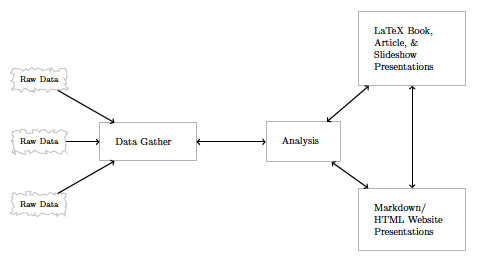
\includegraphics[width=1\linewidth]{imgs/fluxo_gandrud} \end{center}
\end{frame}

\begin{frame}{Dicas}
\protect\hypertarget{dicas}{}
\begin{enumerate}
\item
  Documente tudo!
\item
  Tudo é um arquivo (de texto).
\item
  Todos os arquivos devem ser legíveis (por humanos).
\item
  Relacione explicitamente seus arquivos.
\item
  Tenha um plano para organizar, armazenar e disponibilizar seus
  arquivos.
\end{enumerate}
\end{frame}

\hypertarget{versionando-projetos}{%
\section{Versionando projetos}\label{versionando-projetos}}

\begin{frame}{}
\protect\hypertarget{section-1}{}
\begin{center}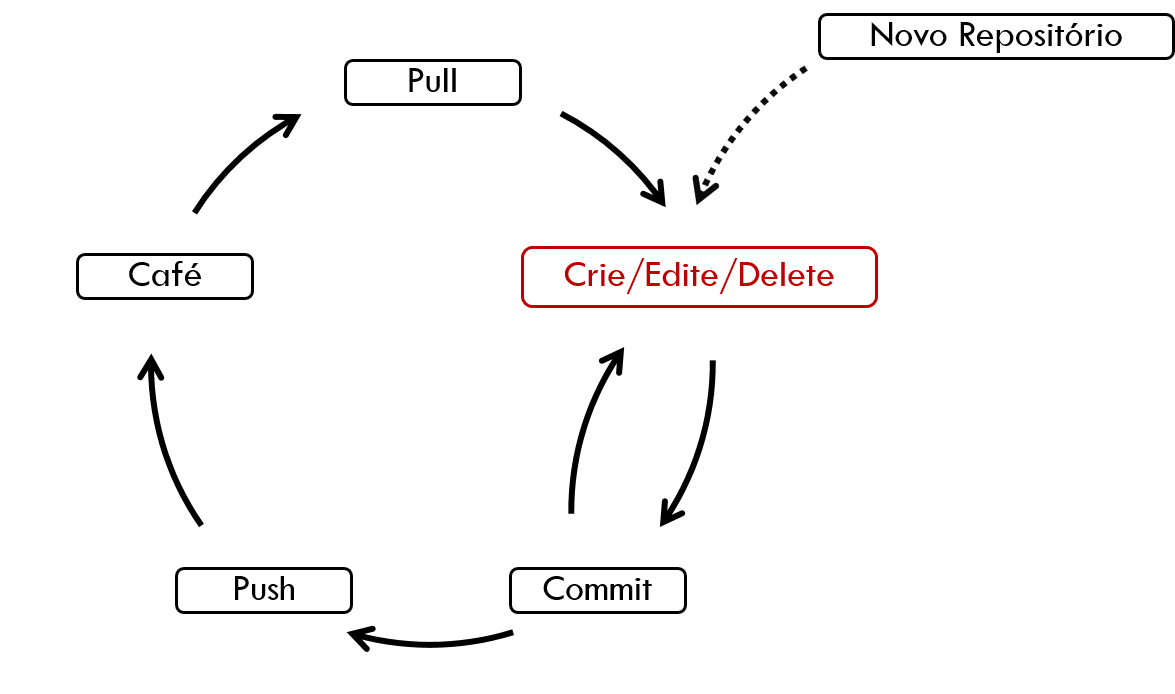
\includegraphics[width=0.8\linewidth]{imgs/fluxo_github_rstudio} \end{center}
\end{frame}

\begin{frame}{Passo-a-passo}
\protect\hypertarget{passo-a-passo}{}
\begin{enumerate}
\item
  Repositório: Criação de repositório do projeto no Github
\item
  .Rproj: Criação do Projeto no RStudio
\item
  Commit: Editando e ``Commitando'' as mudanças no código
\item
  Push: Subindo os commits para o Github
\item
  Pull: Baixando o estado atual do projeto
\end{enumerate}
\end{frame}

\hypertarget{gerenciamento-de-arquivos}{%
\section{Gerenciamento de arquivos}\label{gerenciamento-de-arquivos}}

\hypertarget{ggplot}{%
\section{ggplot}\label{ggplot}}

\begin{frame}{O que você quer mostrar?}
\protect\hypertarget{o-que-vocuxea-quer-mostrar}{}
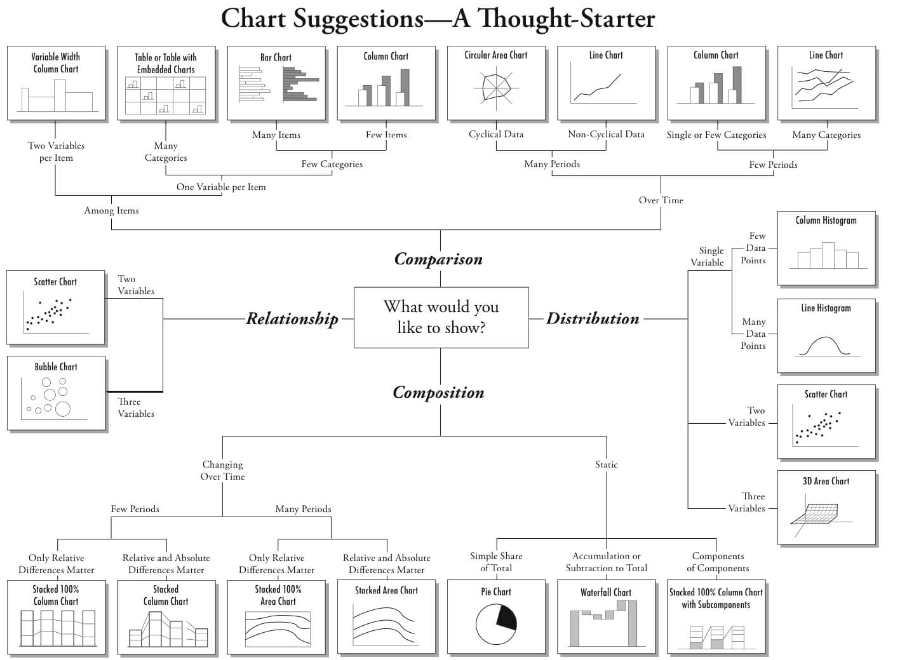
\includegraphics{imgs/Pic_2.png}
\end{frame}

\begin{frame}{Princípios}
\protect\hypertarget{princuxedpios}{}
\begin{itemize}
\item
  O que você quer mostrar?
\item
  Elementos que podem \textbf{destacar} ou \textbf{confundir} o que você
  quer mostrar.
\end{itemize}

-- Exemplo Codeplan

\begin{itemize}
\tightlist
\item
  vamos tentar alternar ``teoria'' com live code
\end{itemize}
\end{frame}

\begin{frame}{Recursos}
\protect\hypertarget{recursos}{}
\begin{itemize}
\item
  R Cookbook \url{http://www.cookbook-r.com/Graphs/}
\item
  STHDA
  \url{http://www.sthda.com/english/wiki/be-awesome-in-ggplot2-a-practical-guide-to-be-highly-effective-r-software-and-data-visualization}
\item
  R Graph Gallery \url{https://www.r-graph-gallery.com/}
\item
  Extensões \url{http://www.ggplot2-exts.org/}
\end{itemize}
\end{frame}

\begin{frame}{Elementos do ggplot}
\protect\hypertarget{elementos-do-ggplot}{}
\begin{itemize}
\item
  Dados
\item
  Geometrias
\item
  Estéticas
\item
  Escalas (estética)
\item
  Escalas (eixos)
\item
  Tema
\item
  Facet
\end{itemize}
\end{frame}

\begin{frame}{Dados \texttt{data\ =}}
\protect\hypertarget{dados-data}{}
\begin{itemize}
\item
  Dado empilhado?
\item
  Cada coluna será uma entrada!
\end{itemize}
\end{frame}

\begin{frame}[fragile]{Geometrias \texttt{geom\_}}
\protect\hypertarget{geometrias-geom_}{}
\begin{itemize}
\item
  geom\_\texttt{tipo\_de\_geometria}
\item
  Recursos +
\item
  cheat sheet
  \url{https://www.rstudio.com/wp-content/uploads/2016/03/ggplot2-cheatsheet-portuguese.pdf}
\item
  manual ggplot \url{https://ggplot2.tidyverse.org/reference/}
\end{itemize}
\end{frame}

\begin{frame}[fragile]{Estéticas \texttt{aes()}}
\protect\hypertarget{estuxe9ticas-aes}{}
\begin{itemize}
\item
  \texttt{x} (\texttt{xmax} e \texttt{xmin})
\item
  \texttt{y}
\item
  \texttt{color}
\item
  \texttt{fill}
\item
  \texttt{shape}
\item
  \texttt{group}
\item
  \texttt{size}
\end{itemize}
\end{frame}

\begin{frame}[fragile]{Escalas (estética) \texttt{scale\_}}
\protect\hypertarget{escalas-estuxe9tica-scale_}{}
\begin{itemize}
\item
  \texttt{scale\_color\_xx}
\item
  \texttt{scale\_fill\_xx}
\item
  \texttt{scale\_shape\_xx}
\end{itemize}
\end{frame}

\begin{frame}[fragile]{Escalas (eixos) \texttt{scale\_x}}
\protect\hypertarget{escalas-eixos-scale_x}{}
\begin{itemize}
\item
  Contínua \texttt{scale\_x\_continuous}
\item
  Discreta \texttt{scale\_x\_discrete}
\item
  Série de tempo \texttt{zoo} --\textgreater{} \texttt{scale\_yearmon}
\end{itemize}
\end{frame}

\begin{frame}[fragile]{Tema}
\protect\hypertarget{tema}{}
\begin{itemize}
\item
  Customização total da visualização
\item
  Eixos
\item
  Texto \texttt{element\_text}
\item
  linhas de grade
\end{itemize}
\end{frame}

\begin{frame}{Facet}
\protect\hypertarget{facet}{}
\begin{itemize}
\item
  facet\_grid
\item
  facet\_wrap
\end{itemize}
\end{frame}

\begin{frame}{Gráficos com interatividade}
\protect\hypertarget{gruxe1ficos-com-interatividade}{}
\begin{itemize}
\item
  ggiraph
\item
  plotly (ggplotly)
\end{itemize}
\end{frame}

\begin{frame}[fragile]{Exercício}
\protect\hypertarget{exercuxedcio}{}
\begin{itemize}
\item
  Carregue os dados de exemplo do pacote survey \texttt{data(api)}, use
  o data.frame \texttt{apisrs}
\item
  Crie o objeto tbl\_svy \texttt{amostra\_expandida} expandindo a
  amostra aleatória simples usando apenas a variável (coluna) ``pw'',
  contendo o peso amostral. Dica: execute
  \texttt{as\_survey(weight=pw)}.
\item
  Usando a variável \texttt{stype} crie uma nova variável indicando se a
  escola é de nível fundamental (categorias \textbf{E} e \textbf{M} de
  \texttt{stype}) ou de nível médio (categoria \emph{H} de
  \texttt{stype}). Dica: use \texttt{mutate}e \texttt{case\_when}.
\item
  Faça um gráfico de barras comparando a variação média das notas de
  1999 (\texttt{api99}) e 2000 (\texttt{api00}) por nível e utilize as
  estimativas intervalares. Dica: olhe o código da aula 07, utilize
  \texttt{geom\_errorbar} para a estimativa intervalar.
\end{itemize}
\end{frame}

\begin{frame}[fragile]{Resolução}
\protect\hypertarget{resoluuxe7uxe3o}{}
\begin{Shaded}
\begin{Highlighting}[]
\KeywordTok{data}\NormalTok{(api)}

\NormalTok{amostra\_expandida \textless{}{-}}\StringTok{ }\NormalTok{apisrs }\OperatorTok{\%\textgreater{}\%}\StringTok{ }
\StringTok{  }\KeywordTok{as\_survey}\NormalTok{(}\DataTypeTok{weight =}\NormalTok{ pw) }\OperatorTok{\%\textgreater{}\%}
\StringTok{  }\KeywordTok{mutate}\NormalTok{(}\DataTypeTok{nivel=}\KeywordTok{case\_when}\NormalTok{(}
\NormalTok{    stype}\OperatorTok{==}\StringTok{"E"}\OperatorTok{\textasciitilde{}}\StringTok{"Fundamental"}\NormalTok{,}
\NormalTok{    stype}\OperatorTok{==}\StringTok{"M"}\OperatorTok{\textasciitilde{}}\StringTok{"Fundamental"}\NormalTok{,}
\NormalTok{    stype}\OperatorTok{==}\StringTok{"H"}\OperatorTok{\textasciitilde{}}\StringTok{"Médio"}
\NormalTok{  ))}
\end{Highlighting}
\end{Shaded}
\end{frame}

\begin{frame}[fragile]{}
\protect\hypertarget{section-2}{}
\begin{Shaded}
\begin{Highlighting}[]
\NormalTok{out \textless{}{-}}\StringTok{ }\NormalTok{amostra\_expandida }\OperatorTok{\%\textgreater{}\%}
\StringTok{  }\KeywordTok{group\_by}\NormalTok{(nivel) }\OperatorTok{\%\textgreater{}\%}
\StringTok{  }\KeywordTok{summarise}\NormalTok{(}\DataTypeTok{api\_diff =} 
              \KeywordTok{survey\_mean}\NormalTok{(api00 }\OperatorTok{{-}}\StringTok{ }\NormalTok{api99, }\DataTypeTok{vartype =} \StringTok{"ci"}\NormalTok{))}
\end{Highlighting}
\end{Shaded}
\end{frame}

\begin{frame}[fragile]{}
\protect\hypertarget{section-3}{}
\begin{Shaded}
\begin{Highlighting}[]
\NormalTok{grafico \textless{}{-}}\StringTok{ }\NormalTok{out }\OperatorTok{\%\textgreater{}\%}\StringTok{ }
\StringTok{  }\KeywordTok{ggplot}\NormalTok{(}\KeywordTok{aes}\NormalTok{(}\DataTypeTok{x =}\NormalTok{ nivel, }\DataTypeTok{y =}\NormalTok{ api\_diff, }
             \DataTypeTok{fill =}\NormalTok{ nivel,}\DataTypeTok{color=}\NormalTok{nivel,}
                       \DataTypeTok{ymax =}\NormalTok{ api\_diff\_upp, }
             \DataTypeTok{ymin =}\NormalTok{ api\_diff\_low)) }\OperatorTok{+}
\StringTok{  }\KeywordTok{geom\_bar}\NormalTok{(}\DataTypeTok{stat =} \StringTok{"identity"}\NormalTok{,}\DataTypeTok{alpha=}\FloatTok{0.6}\NormalTok{) }\OperatorTok{+}
\StringTok{  }\KeywordTok{geom\_errorbar}\NormalTok{(}\DataTypeTok{width =} \DecValTok{0}\NormalTok{,}\DataTypeTok{size=}\DecValTok{3}\NormalTok{) }
\end{Highlighting}
\end{Shaded}
\end{frame}

\begin{frame}[fragile]{}
\protect\hypertarget{section-4}{}
\begin{Shaded}
\begin{Highlighting}[]
\NormalTok{grafico}
\end{Highlighting}
\end{Shaded}

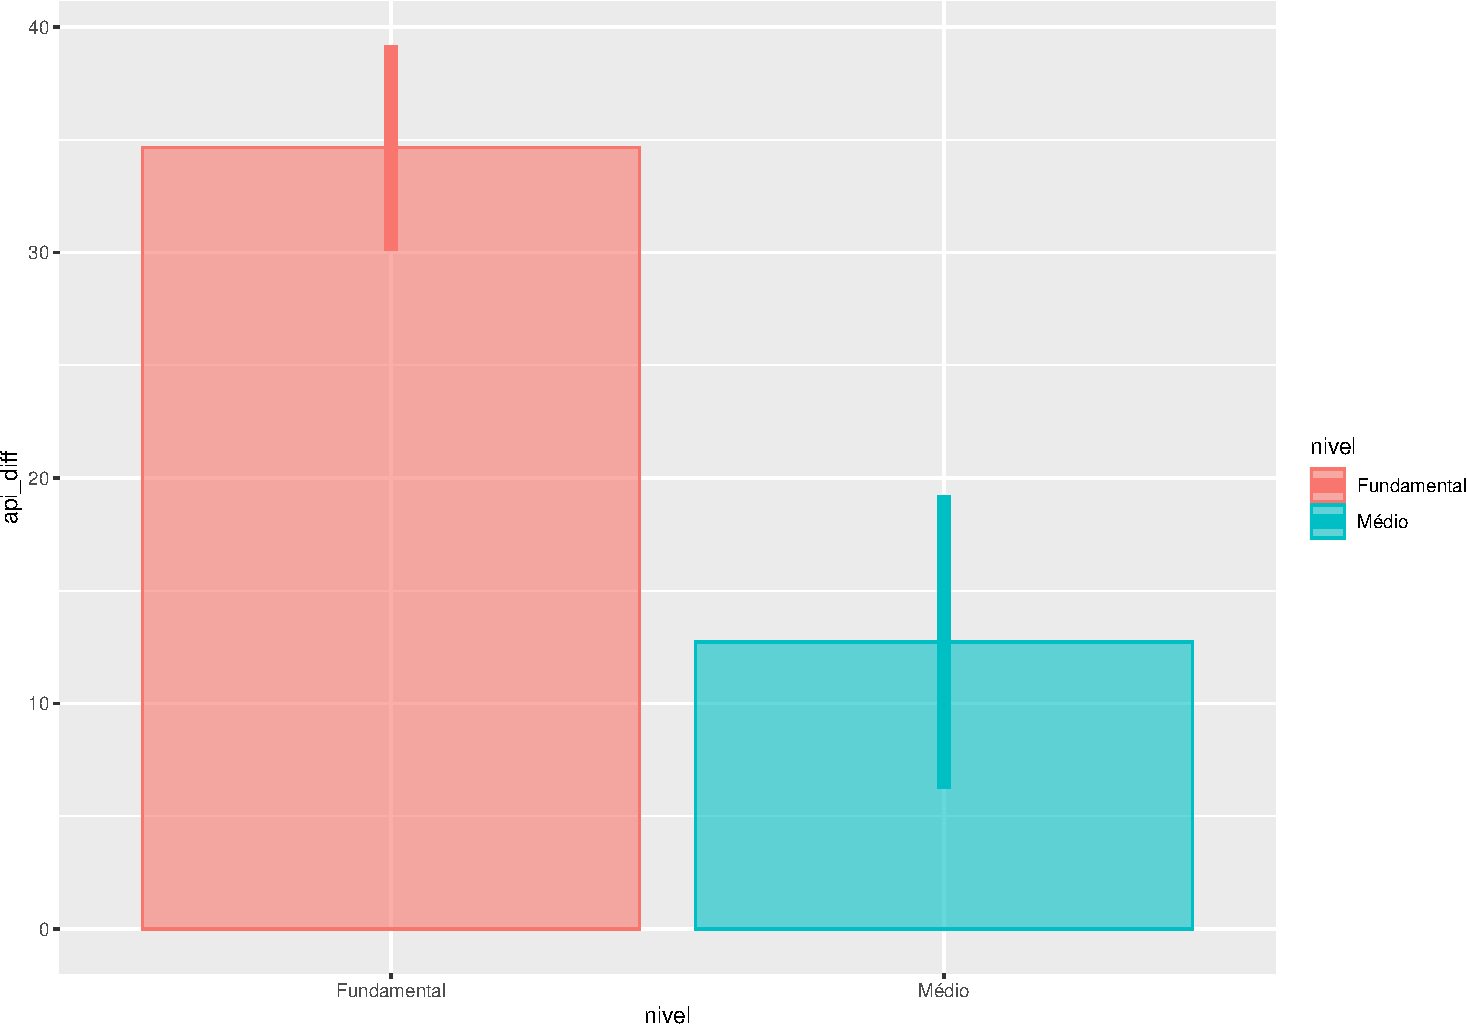
\includegraphics{aula_05_files/figure-beamer/unnamed-chunk-7-1.pdf}
\end{frame}

\end{document}
